\section{Полнота пространства $ C[a,b] $, неполнота пространств непрерывных на отрезке функций с интегральными нормами.}

\begin{greyTheorem}
	Пространство $ \mathcal{C}[a,b] $ полно, а пространства $ \mathcal{L}_C^1[a,b] $ и $ \mathcal{L}_C^2[a,b] $ неполны.
\end{greyTheorem}
\begin{greyProof}
	Если последовательность $ f_n $ непрерывных на $ [a,b] $ функций фундаментальная в норме $ ||\circ||_C $, то 
	\[
		\forall \varepsilon > 0 \rightarrow \exists n_0: \forall n,m \geqslant n_0, \forall x \in [a,b] \mapsto |f_n(x) - f_m(x)| < \varepsilon
	\]
	т.е. выполнен критерий Коши равномерной сходимости, и $ f_n(x) \rightrightarrows f(x)\text{ на } [a,b]$. Предельная функция для равномерно сходящейся последовательности непрерывных функций также непрерывна, поэтому $ f \in \mathcal{C}[a,b] $. Итак, $ fn \rightarrow f $ в $ \mathcal{C}[a,b] $, и пространство $ \mathcal{C}[a,b]  $ полно.
	
	Докажем неполноту $ \mathcal{L}_C^2[-1,1] $(в общем случае неполнота $ \mathcal{L}_C^2 $ и $ \mathcal{L}_C^1 $ доказывается аналогично). Рассмотрим последовательность непрерывных на $ [-1,1] $ функций
	\[
		f_n(x) = \begin{cases}
		nx, \text{ если } -\frac{1}{n}\leqslant x\leqslant\frac{1}{n}\\
		1, \text{ если } x \in \left[ -1;-\frac{1}{n} \right] \cup \left[ \frac{1}{n}; 1 \right]
		\end{cases}
	\]
	График такой функции:
	
\begin{minipage}{0.4\linewidth}
	\begin{figure}[H]
		\centering
		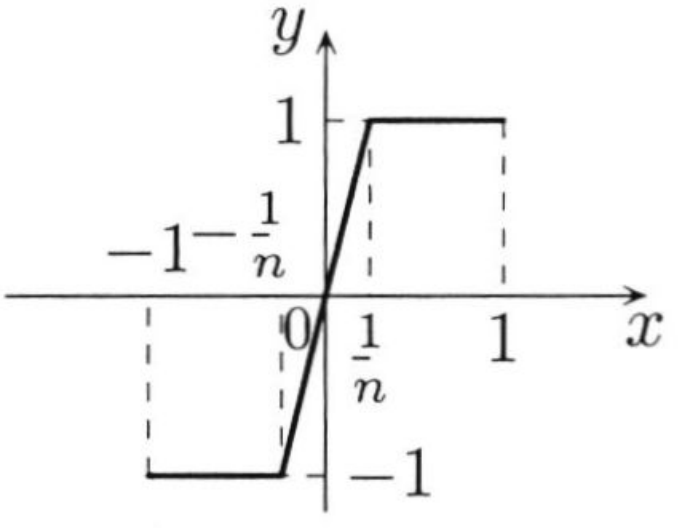
\includegraphics[width=\linewidth]{pic1.png}
	\end{figure}
\end{minipage}
~
\begin{minipage}{0.6\linewidth}
Легко видеть, что
\[
	\forall x \in [0,1] \rightarrow \lim\limits_{n \rightarrow \infty} f_n(x) = \text{sign }x = f(x)  
\]
Докажем, что имеет место сходимость также в среднем квадратичном($ \text{sign }x \in \mathcal{L}_R^2[-1,1 $). В самом деле,
\begin{multline*}
	||f_n - f||_2^2 = \int_{-1}^1 (f_n(x) - f(x))^2dx =\\= 2\int_{0}^{\frac{1}{n}}(1-nx)^2dx < 2\int_{0}^{\frac{1}{n}}1dx = \dfrac{2}{n} \rightarrow 0
\end{multline*}
то есть $ ||f_n-f||_2 \rightarrow0 $
\end{minipage}
\end{greyProof}
\begin{greyEmpty}
Поэтому последовательность $ f_n $ фундаментальна в $ \mathcal{L}_R^2[-1,1] $, значит, и в $ \mathcal{L}_C^2[-1,1] $. Но она не может сходиться в $ \mathcal{L}_C^2[-1,1] $, так как не существует непрерывной на $ [-1,1] $ функции $ g $ такой, что $ ||f_n-g||_2 \rightarrow 0 $.В самом деле, если $ f_n \rightarrow g $ в $ \mathcal{L}_C^2[-1,1] $, то $ f_n \rightarrow g $ в $ \mathcal{L}_R^2[-1,1]$. Так как последовательность $ f_n $ имеет в $ \mathcal{L}_R^2[-1,1] $ два передела $ f $ и $ g $, то $ f =g $ в $ \mathcal{L}_R^2[-1,1] $, т.е. $ f\sim g $ и $ \int_{-1}^1 (f(x) - g(x))^2 dx = 0 $. Отсюда следует, что $ \int_{0}^1 (f(x)-g(x))^2dx = 0 $. Так как $ f(x) = 1 $ на $ [0,1] $, то $ \int_{0}^1(1-g(x))^2dx = 0 $. Так как функция $ g $ непрерывна на $ [-1,1] $, то $ g(x) \equiv 1 $ на $ [0,1] $.Аналогично $ g(x) \equiv -1 $ на $ [-1,0] $. Полученное противоречие показывает, что фундаментальная последовательность $ f_n $ в $ \mathcal{L}_C^2[-1,1] $ не имеет предела в этом пространстве, т.е. пространство $ \mathcal{L}_C^2[-1,1] $ неполно.
\end{greyEmpty}